

\tikzset{every picture/.style={line width=0.75pt}} %set default line width to 0.75pt        

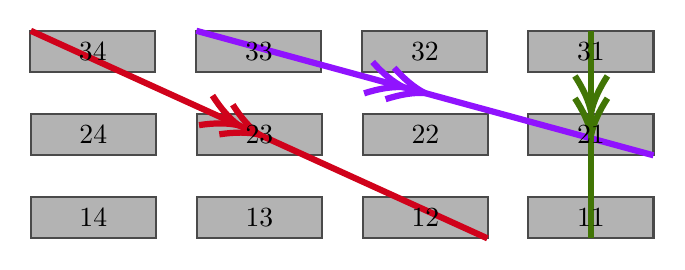
\begin{tikzpicture}[x=0.75pt,y=0.75pt,yscale=-1,xscale=1]
%uncomment if require: \path (0,300); %set diagram left start at 0, and has height of 300

%Shape: Rectangle [id:dp9677752234257792] 
\draw  [color={rgb, 255:red, 74; green, 74; blue, 74 }  ,draw opacity=1 ][fill={rgb, 255:red, 155; green, 155; blue, 155 }  ,fill opacity=0.76 ] (119.76,50) -- (180,50) -- (180,70) -- (119.76,70) -- cycle ;
%Shape: Rectangle [id:dp7783045174475527] 
\draw  [color={rgb, 255:red, 74; green, 74; blue, 74 }  ,draw opacity=1 ][fill={rgb, 255:red, 155; green, 155; blue, 155 }  ,fill opacity=0.76 ] (199.76,50) -- (260,50) -- (260,70) -- (199.76,70) -- cycle ;
%Shape: Rectangle [id:dp2916565511058188] 
\draw  [color={rgb, 255:red, 74; green, 74; blue, 74 }  ,draw opacity=1 ][fill={rgb, 255:red, 155; green, 155; blue, 155 }  ,fill opacity=0.76 ] (279.76,50) -- (340,50) -- (340,70) -- (279.76,70) -- cycle ;
%Shape: Rectangle [id:dp6887263347251699] 
\draw  [color={rgb, 255:red, 74; green, 74; blue, 74 }  ,draw opacity=1 ][fill={rgb, 255:red, 155; green, 155; blue, 155 }  ,fill opacity=0.76 ] (359.76,50) -- (420,50) -- (420,70) -- (359.76,70) -- cycle ;
%Shape: Rectangle [id:dp7312242099062684] 
\draw  [color={rgb, 255:red, 74; green, 74; blue, 74 }  ,draw opacity=1 ][fill={rgb, 255:red, 155; green, 155; blue, 155 }  ,fill opacity=0.76 ] (359.76,90) -- (420,90) -- (420,110) -- (359.76,110) -- cycle ;
%Shape: Rectangle [id:dp3236731708710169] 
\draw  [color={rgb, 255:red, 74; green, 74; blue, 74 }  ,draw opacity=1 ][fill={rgb, 255:red, 155; green, 155; blue, 155 }  ,fill opacity=0.76 ] (359.76,130) -- (420,130) -- (420,150) -- (359.76,150) -- cycle ;
%Shape: Rectangle [id:dp46880323529823853] 
\draw  [color={rgb, 255:red, 74; green, 74; blue, 74 }  ,draw opacity=1 ][fill={rgb, 255:red, 155; green, 155; blue, 155 }  ,fill opacity=0.76 ] (280,130) -- (340.24,130) -- (340.24,150) -- (280,150) -- cycle ;
%Shape: Rectangle [id:dp7337467153729857] 
\draw  [color={rgb, 255:red, 74; green, 74; blue, 74 }  ,draw opacity=1 ][fill={rgb, 255:red, 155; green, 155; blue, 155 }  ,fill opacity=0.76 ] (280,90) -- (340.24,90) -- (340.24,110) -- (280,110) -- cycle ;
%Shape: Rectangle [id:dp6938832339212349] 
\draw  [color={rgb, 255:red, 74; green, 74; blue, 74 }  ,draw opacity=1 ][fill={rgb, 255:red, 155; green, 155; blue, 155 }  ,fill opacity=0.76 ] (200,90) -- (260.24,90) -- (260.24,110) -- (200,110) -- cycle ;
%Shape: Rectangle [id:dp2812215450878759] 
\draw  [color={rgb, 255:red, 74; green, 74; blue, 74 }  ,draw opacity=1 ][fill={rgb, 255:red, 155; green, 155; blue, 155 }  ,fill opacity=0.76 ] (200,130) -- (260.24,130) -- (260.24,150) -- (200,150) -- cycle ;
%Shape: Rectangle [id:dp7929517313076475] 
\draw  [color={rgb, 255:red, 74; green, 74; blue, 74 }  ,draw opacity=1 ][fill={rgb, 255:red, 155; green, 155; blue, 155 }  ,fill opacity=0.76 ] (120,90) -- (180.24,90) -- (180.24,110) -- (120,110) -- cycle ;
%Shape: Rectangle [id:dp17968757590374962] 
\draw  [color={rgb, 255:red, 74; green, 74; blue, 74 }  ,draw opacity=1 ][fill={rgb, 255:red, 155; green, 155; blue, 155 }  ,fill opacity=0.76 ] (120,130) -- (180.24,130) -- (180.24,150) -- (120,150) -- cycle ;
%Straight Lines [id:da8414412126257806] 
\draw [color={rgb, 255:red, 208; green, 2; blue, 27 }  ,draw opacity=1 ][line width=2.25]    (120,50) -- (340,150) ;
\draw [shift={(230,100)}, rotate = 204.44] [color={rgb, 255:red, 208; green, 2; blue, 27 }  ,draw opacity=1 ][line width=2.25]    (28.22,-7.84) .. controls (21.85,-3.68) and (16.03,-1.07) .. (10.74,0) .. controls (16.03,1.07) and (21.85,3.68) .. (28.22,7.84)(17.49,-7.84) .. controls (11.12,-3.68) and (5.29,-1.07) .. (0,0) .. controls (5.29,1.07) and (11.12,3.68) .. (17.49,7.84)   ;
%Straight Lines [id:da3854874229182752] 
\draw [color={rgb, 255:red, 144; green, 19; blue, 254 }  ,draw opacity=1 ][line width=2.25]    (199.76,50) -- (420,110) ;
\draw [shift={(309.88,80)}, rotate = 195.24] [color={rgb, 255:red, 144; green, 19; blue, 254 }  ,draw opacity=1 ][line width=2.25]    (28.22,-7.84) .. controls (21.85,-3.68) and (16.03,-1.07) .. (10.74,0) .. controls (16.03,1.07) and (21.85,3.68) .. (28.22,7.84)(17.49,-7.84) .. controls (11.12,-3.68) and (5.29,-1.07) .. (0,0) .. controls (5.29,1.07) and (11.12,3.68) .. (17.49,7.84)   ;
%Straight Lines [id:da8454035078662195] 
\draw [color={rgb, 255:red, 65; green, 117; blue, 5 }  ,draw opacity=1 ][line width=2.25]    (390,50) -- (390,150) ;
\draw [shift={(390,100)}, rotate = 270] [color={rgb, 255:red, 65; green, 117; blue, 5 }  ,draw opacity=1 ][line width=2.25]    (28.22,-7.84) .. controls (21.85,-3.68) and (16.03,-1.07) .. (10.74,0) .. controls (16.03,1.07) and (21.85,3.68) .. (28.22,7.84)(17.49,-7.84) .. controls (11.12,-3.68) and (5.29,-1.07) .. (0,0) .. controls (5.29,1.07) and (11.12,3.68) .. (17.49,7.84)   ;

% Text Node
\draw (149.88,60) node   [align=left] {34};
% Text Node
\draw (229.88,60) node   [align=left] {33};
% Text Node
\draw (309.88,60) node   [align=left] {32};
% Text Node
\draw (150.12,100) node   [align=left] {24};
% Text Node
\draw (230.12,100) node   [align=left] {23};
% Text Node
\draw (310.12,100) node   [align=left] {22};
% Text Node
\draw (389.88,100) node   [align=left] {21};
% Text Node
\draw (389.88,60) node   [align=left] {31};
% Text Node
\draw (389.88,140) node   [align=left] {11};
% Text Node
\draw (310.12,140) node   [align=left] {12};
% Text Node
\draw (230.12,140) node   [align=left] {13};
% Text Node
\draw (150.12,140) node   [align=left] {14};


\end{tikzpicture}
